\section{Feature tracking}

For the feature step we decided to implement KLT with a pyramid, this was because the results with KLT were not good enough (figure \ref{fig:comparison-KLP-pyramid1}). Our implementation of the pyramid may not follow a method proposed by an specific author but it is intuitive. Consider a video with frames $I$ of some size $w, h$, and the same video with frames $I’$ of size $w/2, h/2$. Then, if a keypoint has a “movement” of $[u, v]$ in frame $I$, it will have a movement of $[u/2, v/2]$ in frame $I’$, this is util because KLT assumes that the movement between frames is small. Based on this idea we can build a pyramid such that we compute the motion in the highest level (smallest frame) and “translate” this motion to the smallest level (original image). Note that intermediate levels of the pyramid are not used for motion computation. “Translate” means that if the motion at some level is $[u, v]$, then the motion in a lower level (bigger frame scale) the motion is $[2\times u, 2 \times v]$. 

Some implementation details of the tracking include: a bilinear interpolation in the computation of the derivatives, and a smoothing in the highest level of the pyramid. To compute the derivative of a pixel $(x, y)$ we consider:

\begin{equation}
\begin{split}
\frac{\partial f(x, y)}{\partial x} = \frac{f(x+ 1, y) - f(x-1, y)}{2} \\
\frac{\partial f(x, y)}{\partial y} = \frac{f(x, y + 1) - f(x, y - 1)}{2}
\end{split}
\label{eq:partial-derivatives}
\end{equation}

The denominator 2 is important because without it the motion magnitude is divided by 2 in the final estimation.

A comparison between implementation with and without the pyramid is shown in figures \ref{fig:comparison-KLP-pyramid1} and \ref{fig:comparison-KLP-pyramid2}. When pyramids are not used, most of the points are lost when a big movement occurs.

\begin{figure}[!h]
	\hspace{-1cm}
    \minipage{1.1\textwidth}
	\begin{subfigure}{0.33\textwidth}
	  \centering
	  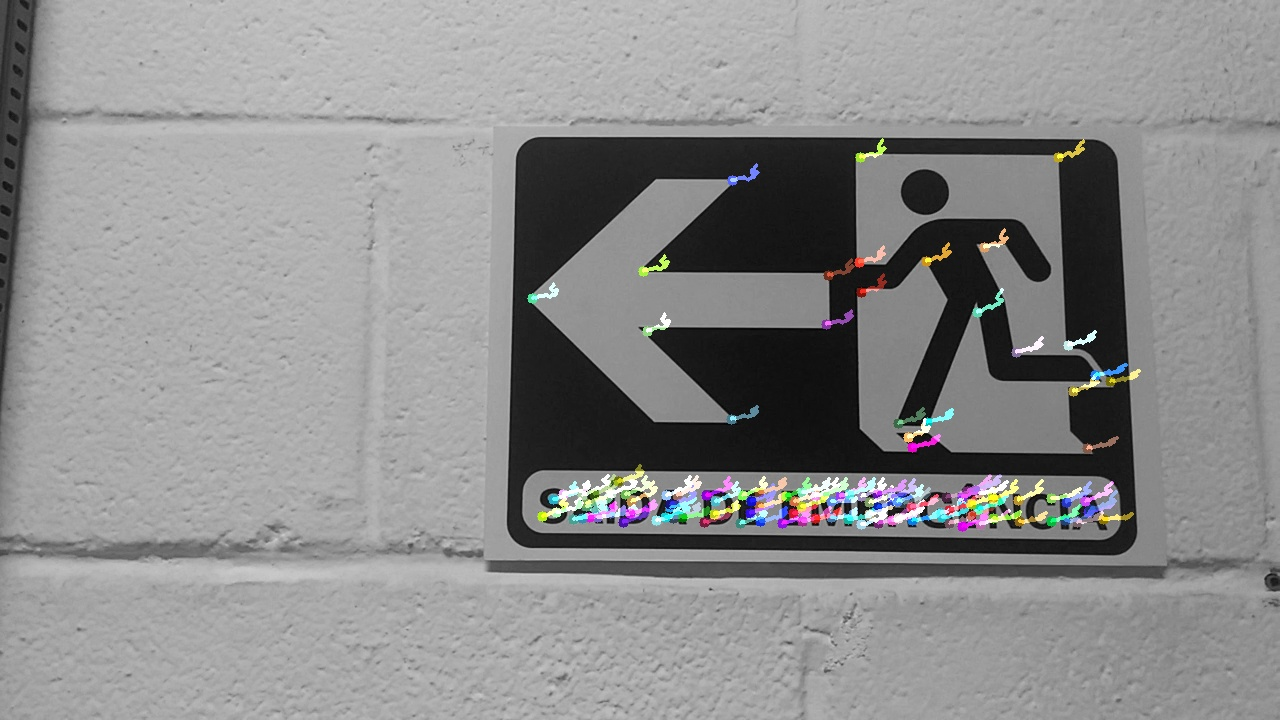
\includegraphics[width=0.99\linewidth]{figs/flowSP-1.jpg}
	\end{subfigure}%
	\begin{subfigure}{0.33\textwidth}
	  \centering
	  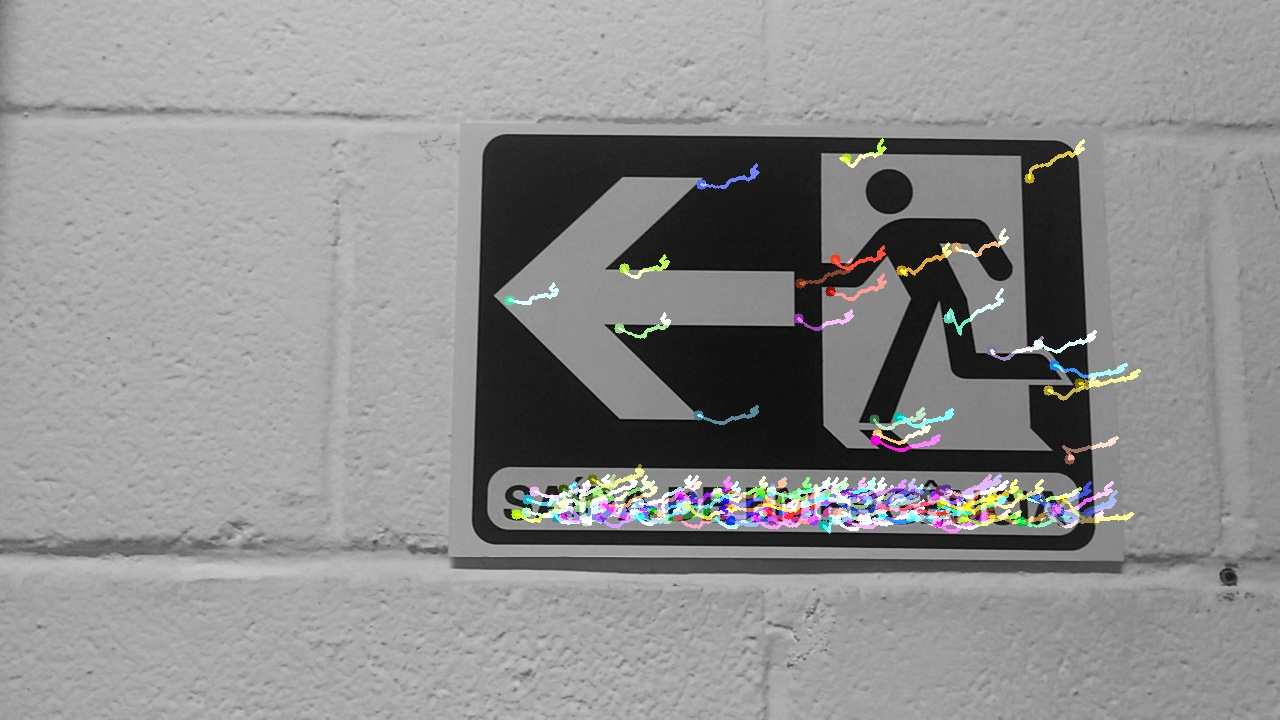
\includegraphics[width=0.99\linewidth]{figs/flowSP-2.jpg}
	\end{subfigure}%
	\begin{subfigure}{0.33\textwidth}
        \centering
      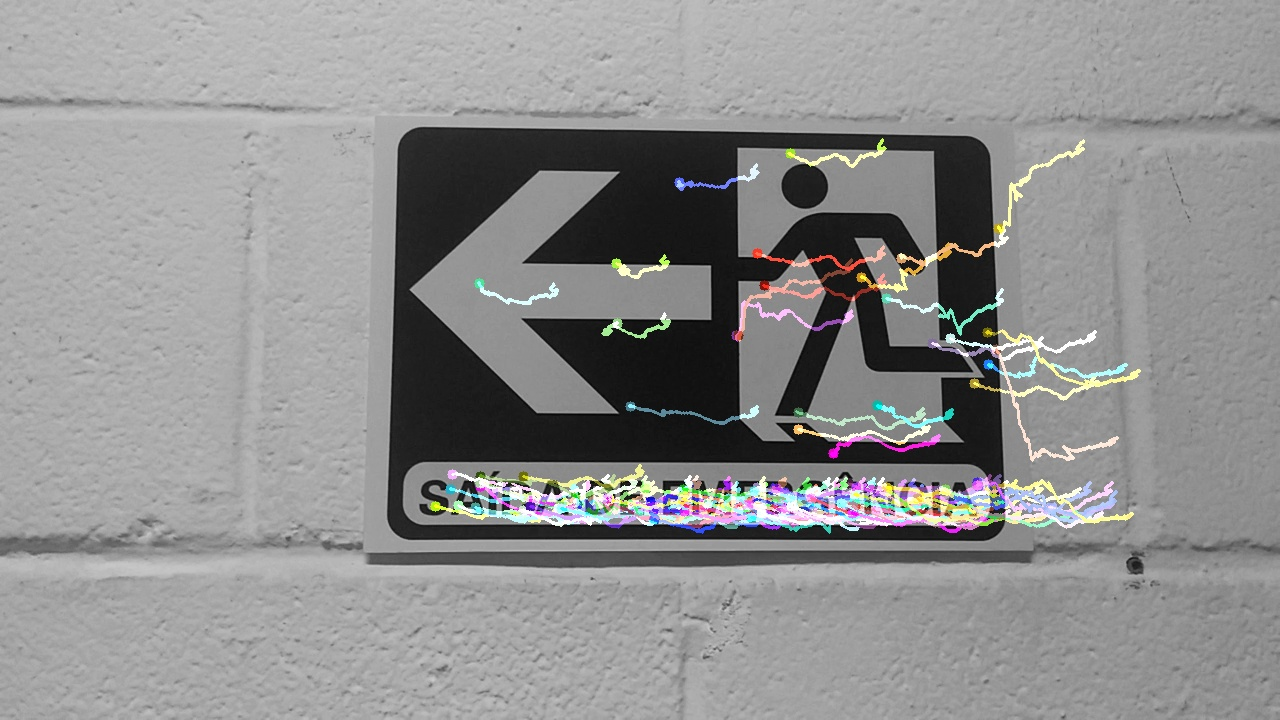
\includegraphics[width=0.99\linewidth]{figs/flowSP-3.jpg}
    \end{subfigure} 
    \endminipage\hfill 
    \caption{KLT without pyramid}
    \label{fig:comparison-KLP-pyramid1}
\end{figure}

\begin{figure}[!h]
    \hspace{-1cm}
    \minipage{1.1\textwidth}
	\begin{subfigure}{0.33\textwidth}
	  \centering
	  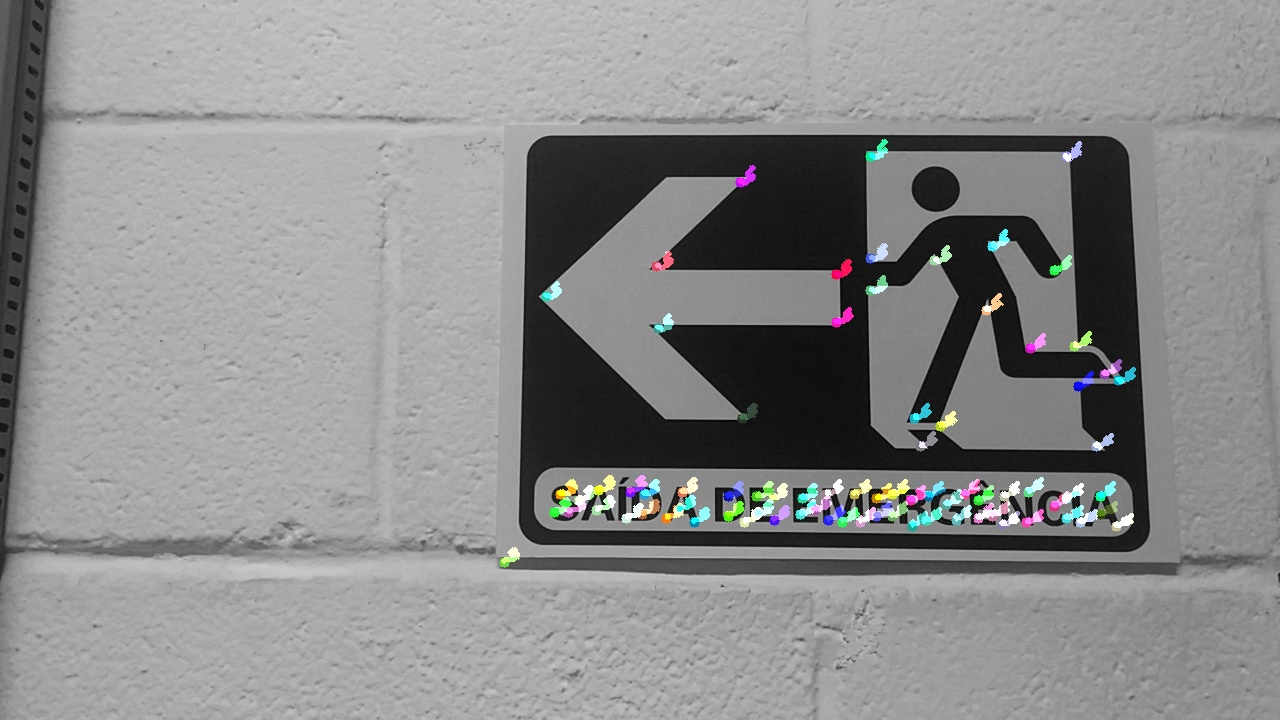
\includegraphics[width=0.99\linewidth]{figs/flow15x15-1.jpg}
	\end{subfigure}%
	\begin{subfigure}{0.33\textwidth}
	  \centering
	  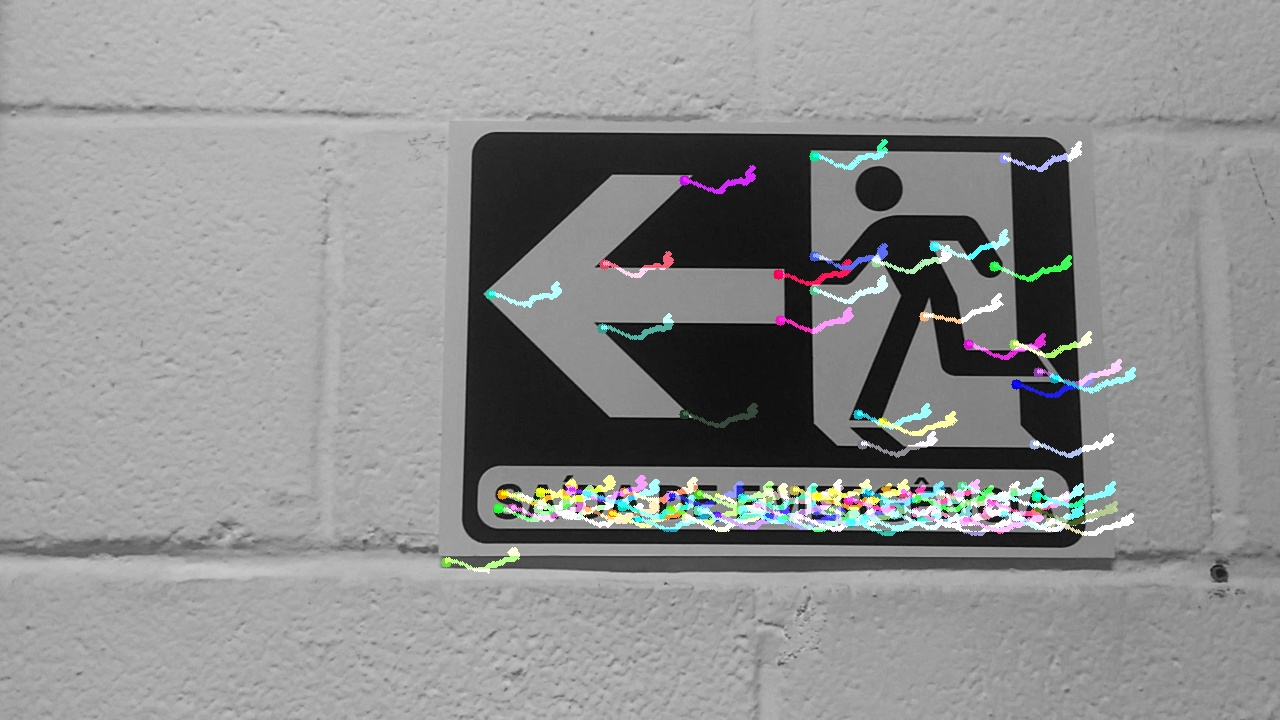
\includegraphics[width=0.99\linewidth]{figs/flow15x15-2.jpg}
	\end{subfigure}%
	\begin{subfigure}{0.33\textwidth}
        \centering
      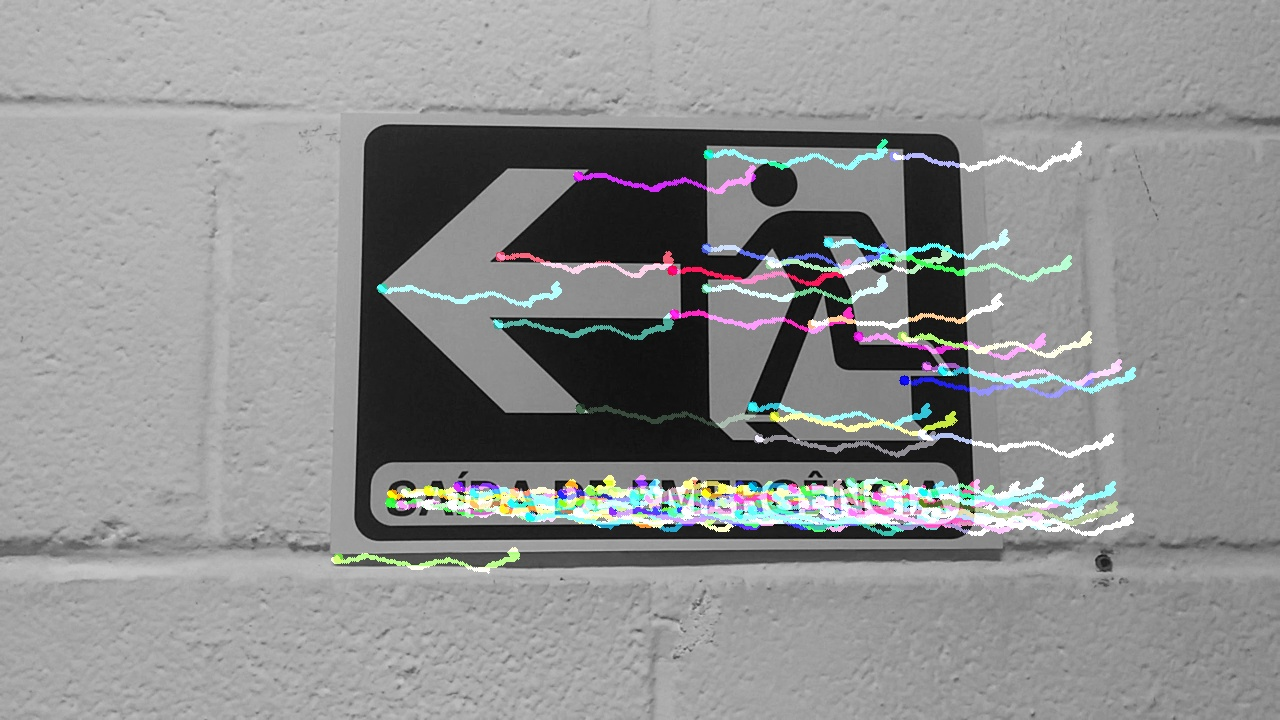
\includegraphics[width=0.99\linewidth]{figs/flow15x15-3.jpg}
    \end{subfigure}  
    \endminipage\hfill
    \caption{KLT with pyramid}    
	\label{fig:comparison-KLP-pyramid2}
\end{figure}

The test of different sizes of neighborhood are shown in figures \ref{fig:comparison-neigh-pyramid1}, \ref{fig:comparison-neigh-pyramid2}, \ref{fig:comparison-neigh-pyramid3}

\begin{figure}[!h]
	\hspace{-1cm}
    \minipage{1.1\textwidth}
	\begin{subfigure}{0.33\textwidth}
	  \centering
	  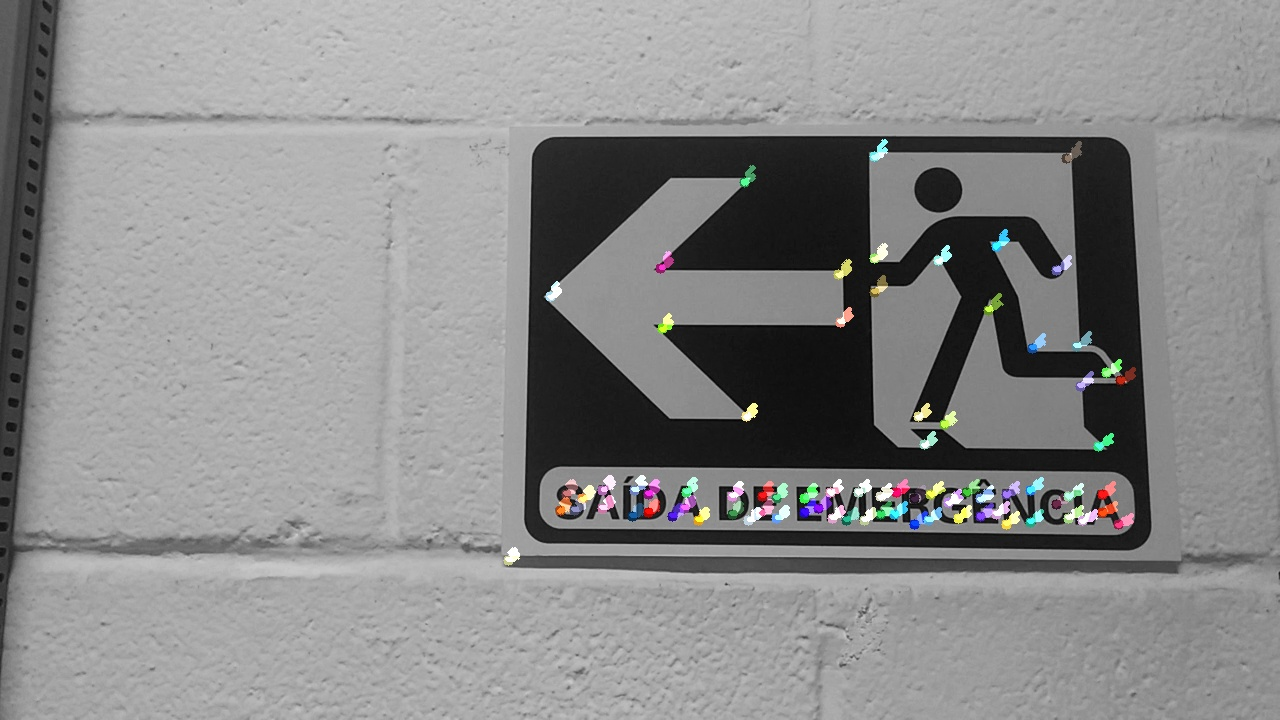
\includegraphics[width=0.99\linewidth]{figs/flow5x5-1.jpg}
	\end{subfigure}%
	\begin{subfigure}{0.33\textwidth}
	  \centering
	  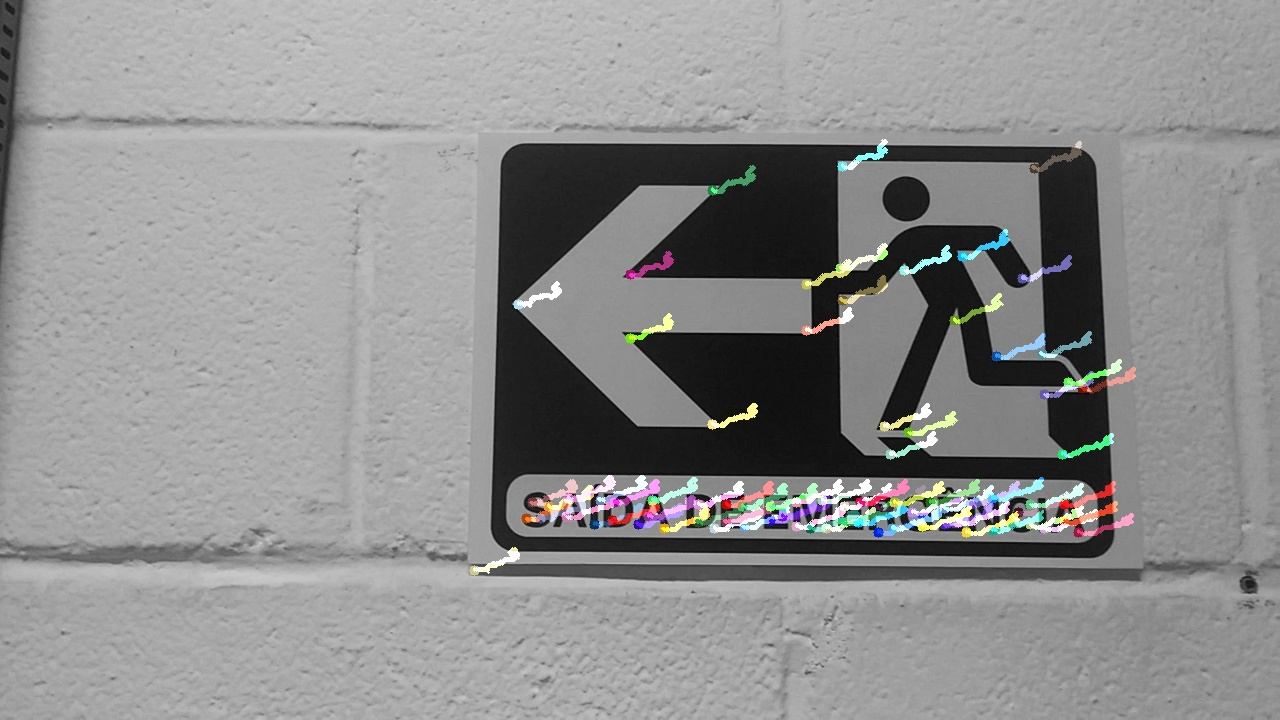
\includegraphics[width=0.99\linewidth]{figs/flow5x5-2.jpg}
	 
	\end{subfigure}%
	\begin{subfigure}{0.33\textwidth}
        \centering
      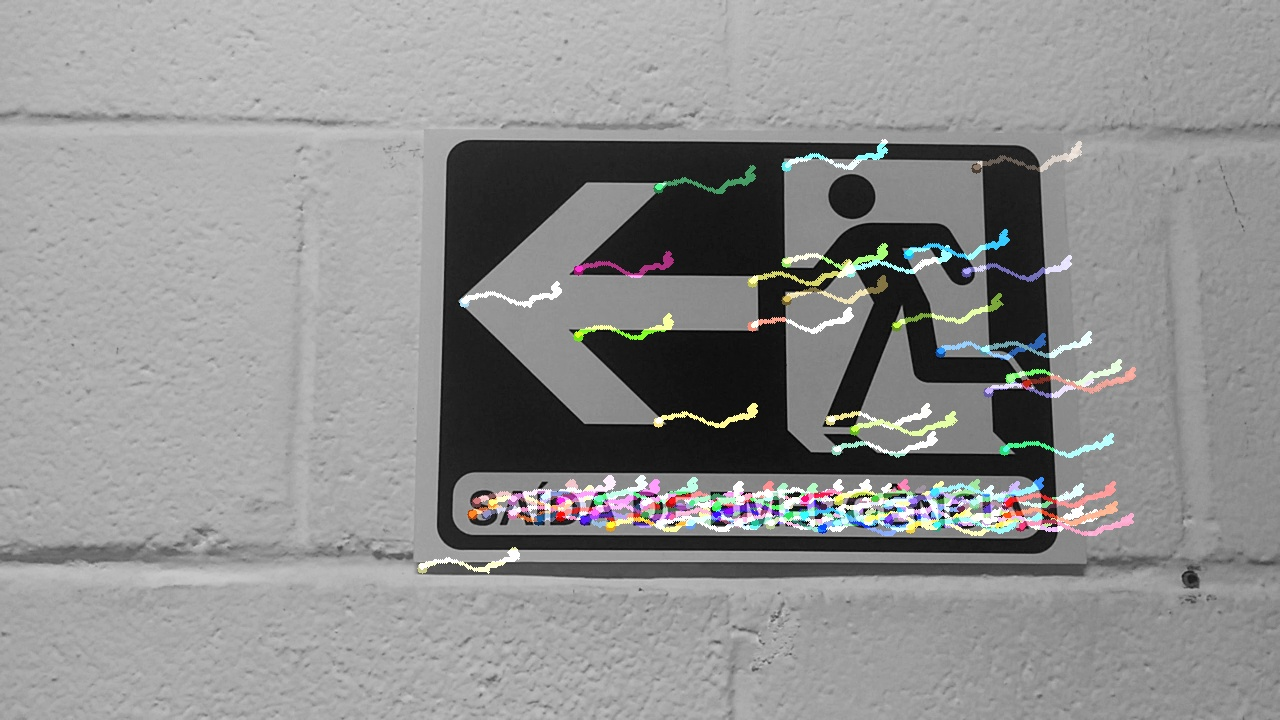
\includegraphics[width=0.99\linewidth]{figs/flow5x5-3.jpg}
    \end{subfigure}
    \endminipage\hfill
    
    \caption{Neightborhood $= 5 \times 5$}
    \label{fig:comparison-neigh-pyramid1}
\end{figure}

\begin{figure}[!h]
   \hspace{-1cm}
    \minipage{1.1\textwidth}
    \centering
	\begin{subfigure}{0.33\textwidth}
	  \centering
	  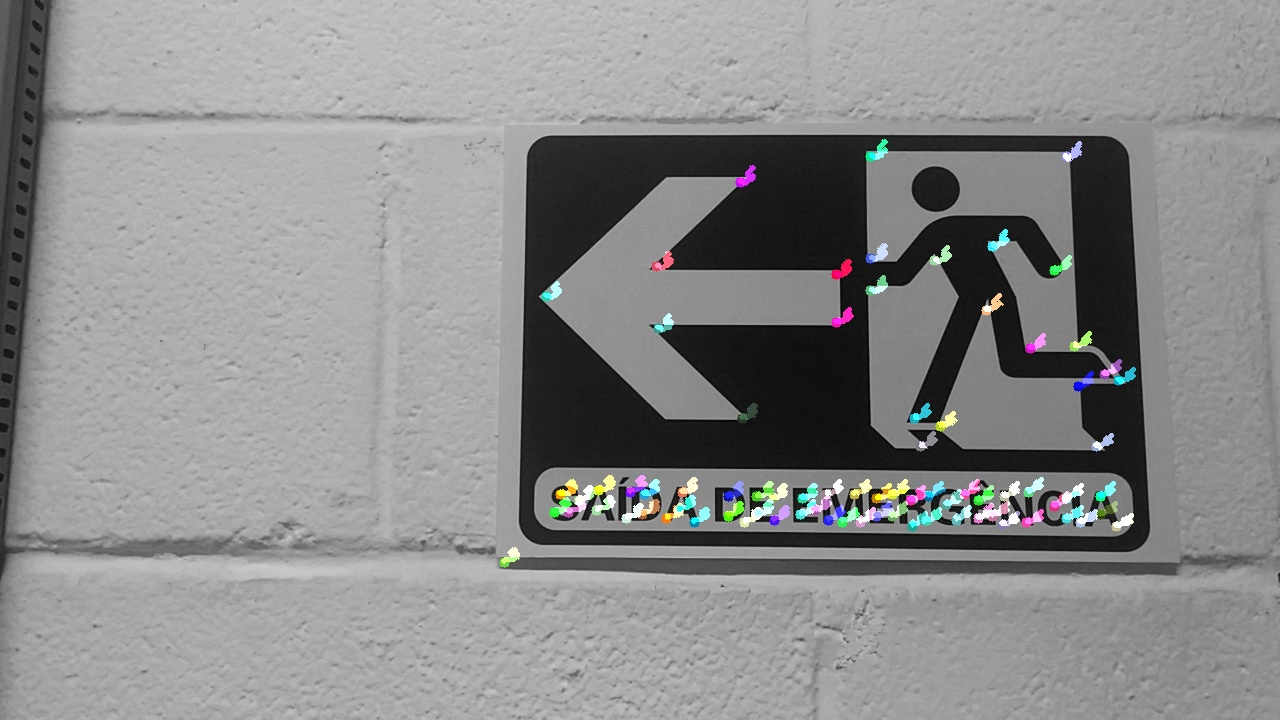
\includegraphics[width=0.99\linewidth]{figs/flow15x15-1.jpg}
	\end{subfigure}%
	\begin{subfigure}{0.33\textwidth}
	  \centering
	  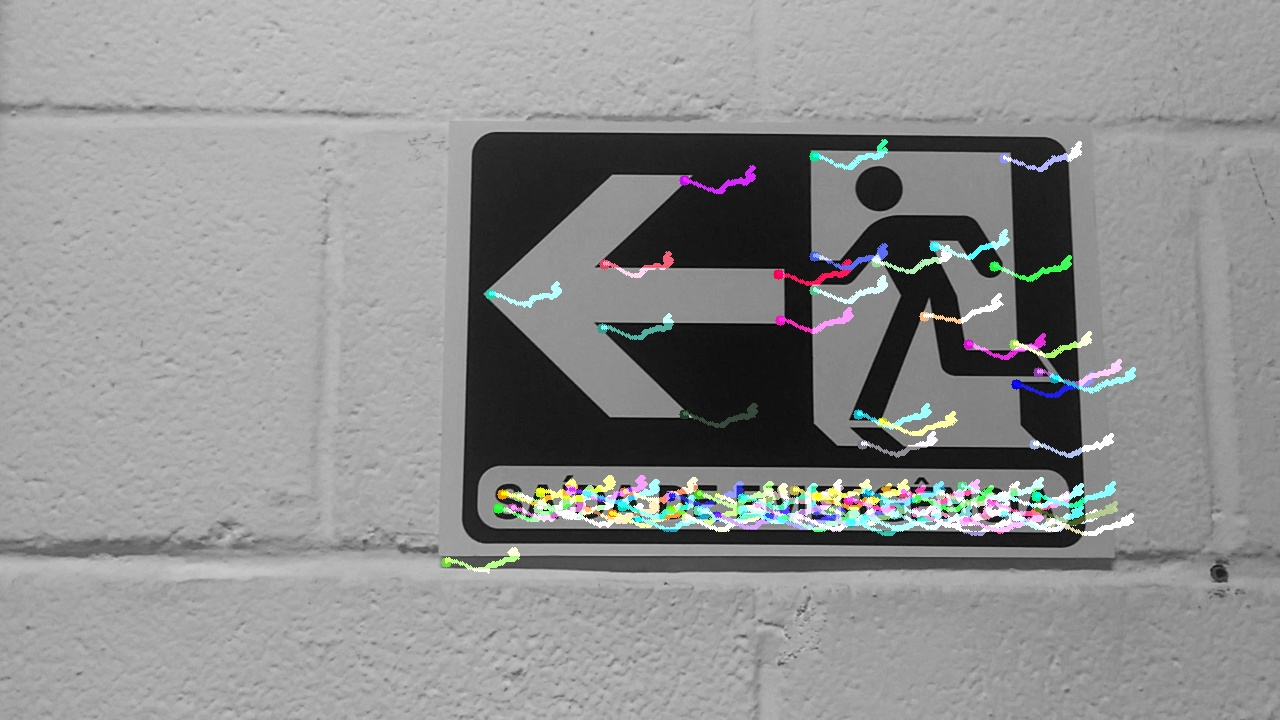
\includegraphics[width=0.99\linewidth]{figs/flow15x15-2.jpg}
	\end{subfigure}%
	\begin{subfigure}{0.33\textwidth}
        \centering
      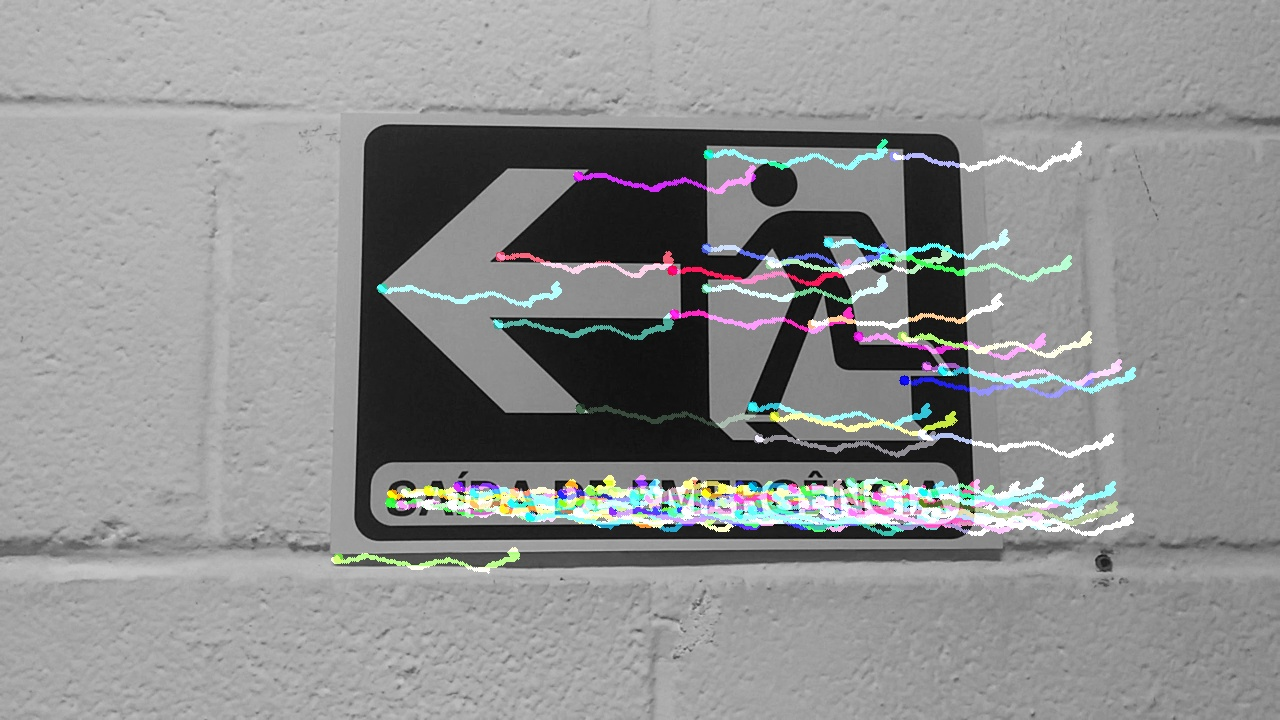
\includegraphics[width=0.99\linewidth]{figs/flow15x15-3.jpg}
    \end{subfigure}

    \endminipage\hfill
        \caption{Neightborhood $= 15 \times 15$}
    \label{fig:comparison-neigh-pyramid2}
\end{figure}

\begin{figure}[!h]
    \hspace{-1cm}
    \minipage{1.1\textwidth}
    \centering
	\begin{subfigure}{0.33\textwidth}
	  \centering
	  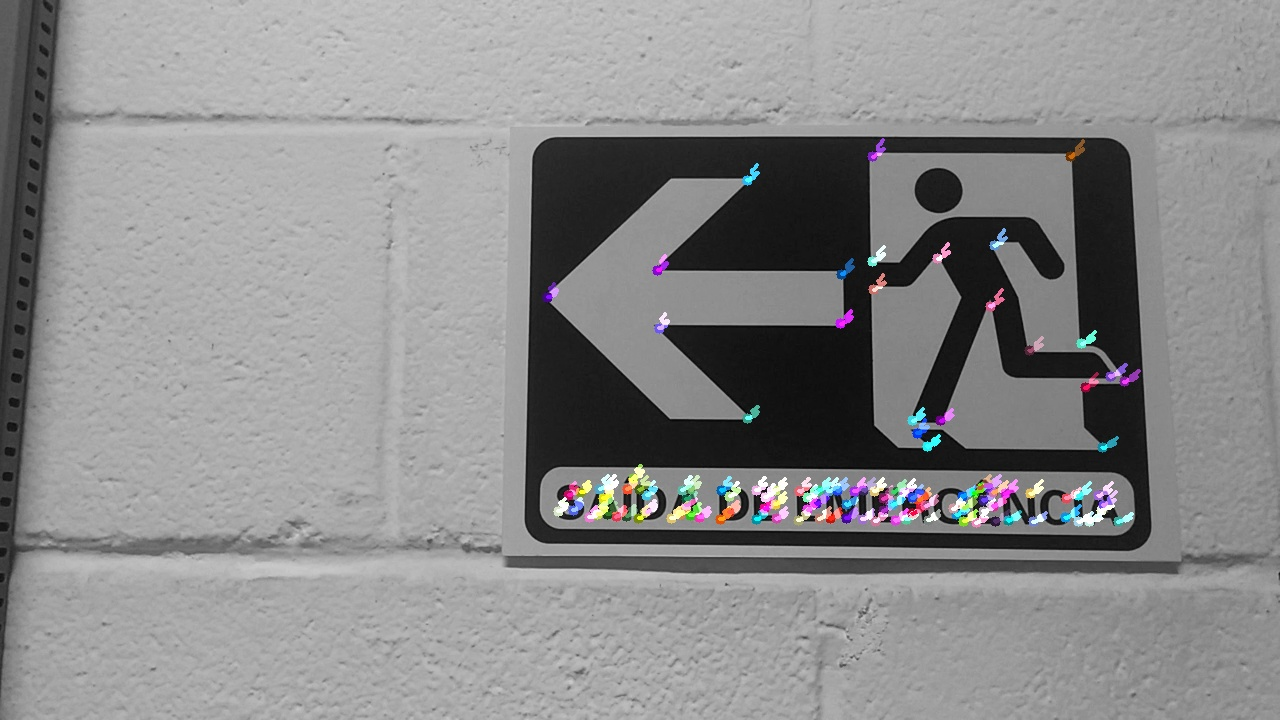
\includegraphics[width=0.99\linewidth]{figs/flow20x20-1.jpg}
	\end{subfigure}%
	\begin{subfigure}{0.33\textwidth}
	  \centering
	  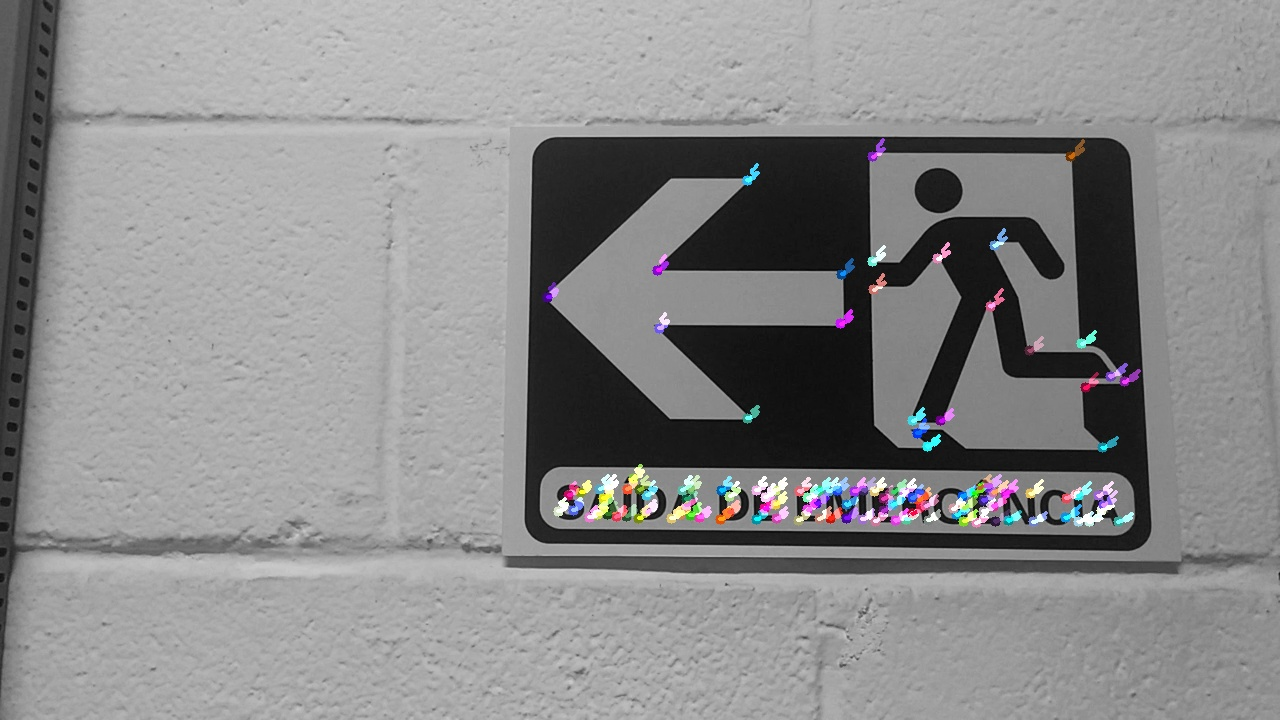
\includegraphics[width=0.99\linewidth]{figs/flow20x20-1.jpg}
	\end{subfigure}%
	\begin{subfigure}{0.33\textwidth}
        \centering
      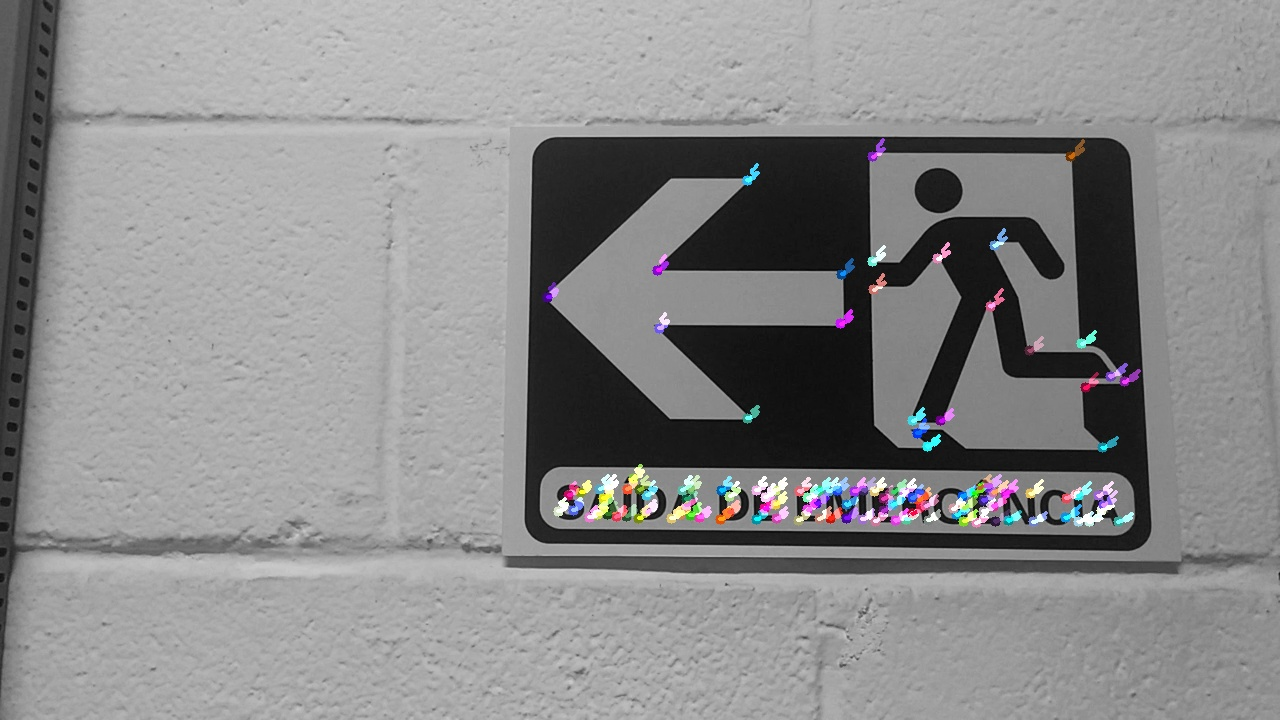
\includegraphics[width=0.99\linewidth]{figs/flow20x20-1.jpg}
    \end{subfigure}
    \endminipage\hfill
    
    \caption{Neightborhood $= 20 \times 20$}
    \label{fig:comparison-neigh-pyramid3}
     
\end{figure}

As can be seen in figures \ref{fig:comparison-neigh-pyramid1}, \ref{fig:comparison-neigh-pyramid2} and \ref{fig:comparison-neigh-pyramid3}, there is not a dramatic improvement with the change of neighborhood, then, we decided to use a $15 \times 15$ neighborhood because the original authors suggest to use this size. Figure \ref{fig:final-tracking} shows the results of tracking of the input video with the $15 \times 15$ neighborhood.


\begin{figure}[!h]
    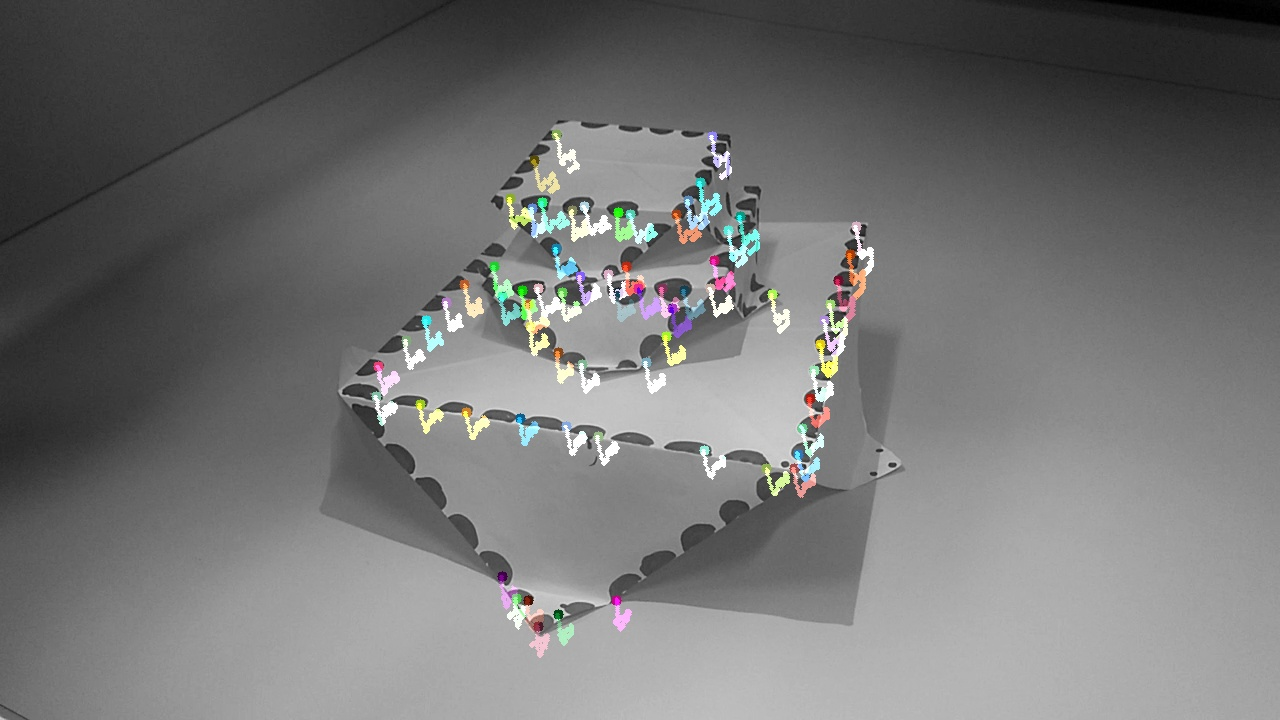
\includegraphics[width=0.99\linewidth]{figs/TrakingPyramid15x15.jpg}
    \caption{Results of tracking}
    \label{fig:final-tracking}
\end{figure}


